\hypertarget{system-thinking-and-system-dynamics}{%
\section{System Thinking and System
Dynamics}\label{system-thinking-and-system-dynamics}}

\hypertarget{causal-loop-diagram}{%
\subsection{Causal Loop Diagram}\label{causal-loop-diagram}}

The following picture shows a casual model of a fish population in a
limited biosphere.

\begin{figure}
\centering
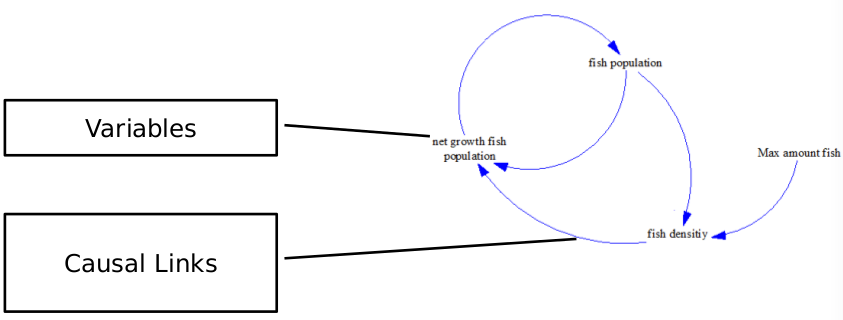
\includegraphics{figures/cld.png}
\caption{CLD}
\end{figure}

\hypertarget{definitions}{%
\subsubsection{Definitions}\label{definitions}}

\textbf{Positive polarity:}\\
Increases (decreases) cause, then increases (decreases) effect.

\textbf{Negative polarity:}\\
Increases (decreases) cause, then decreases (increases) effect.

\textbf{Reinforcing Loop:}\\
The reinforcement increases the initial effect. A loop is reinforced
when the number of minuses is even. e.g.~if I put additional fishes into
the population.

\textbf{Balancing Loop:}\\
The feedback balances the initial effect. A loop is balanced if the
number of minuses are odd.

The following picture shows a casual loop diagram.

\begin{figure}
\centering
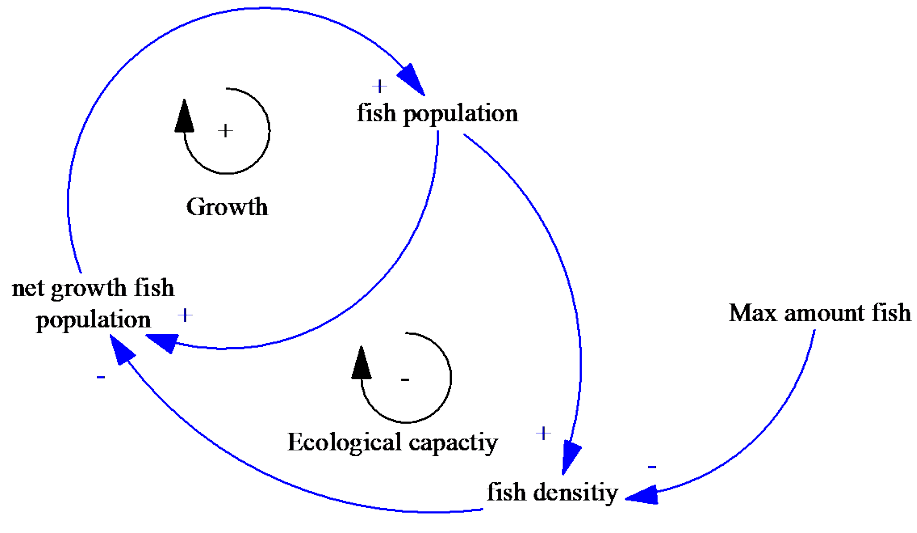
\includegraphics{figures/cldFishpopulation.png}
\caption{CLD}
\end{figure}
